\scanpage{180}
\diagram{\begin{tikzcd}[ampersand replacement=\&,column sep=small,row sep=small]
\ldots\arrow[r]\&\mathbb{R}^i\Gamma_x(F)\arrow[r]\&\unsure{\mathrm{R}|\mathbb{R}}^i\Gamma_X(F)\arrow[r]\&\mathbb{R}^i\Gamma_U(F)\arrow[r]\&\mathbb{R}^{i+1}\Gamma_x(F)\arrow[r]\&\ldots\\
\&\&\times\&\times\&\times\\
\&\mathbb{R}^{-i}\Gamma_X(DF)\&\mathbb{R}^{-i}\Gamma_xDF\arrow[l]\arrow[d]\arrow[dd,bend right=45,no head]\&\mathbb{R}^{-i}\Gamma_U(\unsure{F|DF})\arrow[l]\arrow[d]\arrow[dd,bend left=45,no head]\&\mathbb{R}^{-i-1}\Gamma_XDF\arrow[l]\arrow[d,no head]\arrow[ddl,bend left=20,no head]\&\ldots\arrow[l]\\
\&\&A\&A\&A\\
\&\&\begin{array}{c}\text{dualité parfaite}\\\text{triviale}\\\text{(via \unsure{poncti}\ldots)}\end{array}\&\begin{array}{c}\text{dualité}\\\text{parfaite ??}\end{array}
\end{tikzcd}}
\margin{$f^!\mathbb{R}\mathcal{H}om(F,G)$\par $f^!D=Df^*$}
\margin{$\mathbb{R}\mathcal{H}om(F,G)$\par $D(F\otimes DG)$\par $\mathbb{R}\mathcal{H}om(G,DF)\simeq D(G\overset{\mathbb L}{\otimes}F)$\par $\mathbb{R}\mathcal{H}om(F,D(DG))$\par $\unsure{\mathrm{R}|\mathbb{R}}\mathcal{H}$}
\[
D(H_x^{\unsure{n|i}}(F))\longrightarrow\deleted{\unsure{D\mathcal{H}}}\unsure{\simeq}\mathcal{H}_x^i(DF)_{\unsure{x}}\unsure{\}}
\]
\[
\deleted{\unsure{D}}(F\otimes DG)\simeq D\mathbb{R}\mathcal{H}om(F,\inserted{\unsure{D}}G)
\]
\[
F\longrightarrow DDF
\]
\[
\deleted{H_x^i(F)\longrightarrow}
\]
\figure{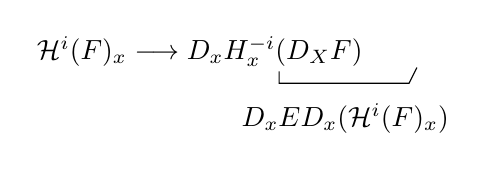
\begin{tikzpicture}[x=1cm,y=1cm]
\node[anchor=west] at (0,0) {$\mathcal{H}^i(F)_x\longrightarrow D_xH_x^{-i}(D_XF)$};
\draw (3.2,-0.25)--(3.2,-0.4)--(4.85,-0.4)--(4.95,-0.2);
\node[anchor=west] at (2.6,-0.85) {$D_x\deleted{\unsure{E}}D_x(\mathcal{H}^i(F)_x)$};
\end{tikzpicture}}
\figure{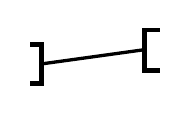
\begin{tikzpicture}[x=1cm,y=1cm]
\draw[line width=1.2pt] (0,0)--(1.3,0.18);\draw[line width=1.7pt] (-0.15,-0.25)--(0,-0.25)--(0,0.25)--(-0.15,0.25);\draw[line width=1.7pt] (1.5,-0.08)--(1.3,-0.08)--(1.3,0.43)--(1.5,0.43);
\end{tikzpicture}}
\margin{$F\otimes DG$\par $-2n,0$}
\figure{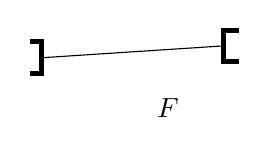
\begin{tikzpicture}[x=1cm,y=1cm]
\draw (0,0)--(2.3,0.15);\draw[line width=1.8pt] (-0.15,-0.2)--(0,-0.2)--(0,0.2)--(-0.15,0.2);\draw[line width=1.8pt] (2.5,-0.05)--(2.3,-0.05)--(2.3,0.35)--(2.5,0.35);
\node[below] at (1.6,-0.4) {$F$};
\end{tikzpicture}}
\figure{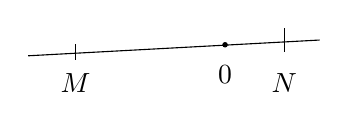
\begin{tikzpicture}[x=1cm,y=1cm]
\draw (-0.4,0)--(3.3,0.2);\draw (0.2,-0.05)--(0.2,0.15);\draw (2.85,0.05)--(2.85,0.35);\fill (2.1,0.14) circle(0.035);
\node[below] at (0.2,-0.1) {$M$};\node[below] at (2.1,0) {$0$};\node[below] at (2.85,-0.1) {$N$};
\end{tikzpicture}}
\figure{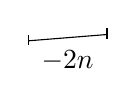
\begin{tikzpicture}[x=1cm,y=1cm]
\draw (0,0)--(1.0,0.08);\draw (0,-0.05)--(0,0.08);\draw (1.0,0.02)--(1.0,0.16);\node[below] at (0.5,0) {$-2n$};
\end{tikzpicture}}
\diagram{\begin{tikzcd}[ampersand replacement=\&,row sep=small]
\text{Tor-dim}_{\unsure{x}}\ F\text{ comprise par }[N,M]\arrow[d,Rightarrow]\\
\text{loc.Inj-dim}^{*}\ D(F)\text{ comprise par }[-2n+N,M]
\end{tikzcd}}
\diagram{\begin{tikzcd}[ampersand replacement=\&,row sep=small]
\text{Inj-dim }F\text{ comprise par }[P,Q]\arrow[d,Rightarrow]\\
\text{Tor-dim }DF\text{ comprise par }[P-2n,Q]
\end{tikzcd}}
\figure{\begin{tikzpicture}[x=1cm,y=1cm]
\node[anchor=west] at (0,0) {$DF\overset{\mathbb L}{\otimes}G\simeq D\mathbb{R}\mathcal{H}om(G,F)$};
\draw (2.95,-0.3)--(2.95,-0.43)--(5.3,-0.43)--(5.4,-0.25);
\node[anchor=west] at (-0.6,-0.8) {$\deleted{DF\otimes DDG\simeq D(F\otimes D\unsure{G})}$};
\node at (4.0,-1.2) {$[P,Q]$};
\draw (2.8,-1.9)--(3.0,-1.9);
\end{tikzpicture}}
\margin{179}
